\documentclass[letterpaper,10pt,notitlepage,fleqn]{article}

\usepackage{nopageno} %gets rid of page numbers
\usepackage{alltt}                                           
\usepackage{float}
\usepackage{color}
\usepackage{url}
\usepackage{balance}
\usepackage[TABBOTCAP, tight]{subfigure}
\usepackage{enumitem}
\usepackage{pstricks, pst-node}
\usepackage{geometry}
\geometry{textheight=9in, textwidth=6.5in} %sets 1" margins 
\newcommand{\cred}[1]{{\color{red}#1}} %command to change font to red
\newcommand{\cblue}[1]{{\color{blue}#1}} % ...blue
\usepackage{hyperref}
\usepackage{textcomp}
\usepackage{listings}
\usepackage{graphicx}

\def\name{Sam Quinn}

\parindent = 0.0 in
\parskip = 0.2 in

\title{Project 3 Write Up}
\author{Sam Quinn}

\begin{document}
\maketitle
\hrule

\section*{Design}

\subsection*{Uniqify.c Program}
Will sort words imputed though standard input or from a text file. This program will then print the sorted word
in alphabetical order with no duplicates via standard output or to a text file.

\begin{itemize} 
\item if no options/arguments, print usage
\item -n is the number of sort processes to use, if not defined the default is 2
\item -i the text file to read unsorted words from, if not defined standard input is default
\item -o the text file to create or append with sorted words if not defined standard output is default
\end{itemize}

\subsection*{Functions of Program Details}

\subsubsection*{-n Option}
The number of sort processes to spawn. This number is limited to 1000 processes by default. With that said high number
of processes exceeding > 500 tend to fail. If user inputs more than more than > 1000 it will print the usage of the
program. The number of processes defined is not the absolute number of processes spawned by this program. The
program spawns a process for the suppressor as well.
\begin{itemize}
\item if there is a number received then spawn that many processes, if no input then 2 is default.
\item NOT RECOMMENDED to use more than 500 processes, but max number is 1000.
\item if more than 1000 is revived print usage
\end{itemize}


\subsubsection*{-i     Option}       
The input file, this file must be in the current directory of the executable. This file must be a text file that
can be read by POSIX read() command. If no input file is designated in the command line Words will be received via
standard input. To close the standard input dialogue you must press Ctrl-D a few times. 
\begin{itemize}
\item if there is a file open it, if not send error.
\item if no file name is received open standard input.
\item Close standard input with Ctrl-D
\end{itemize}

\subsubsection*{-o     Option}
The file in which the sorted words will be saved too. This function will print every word received from input on
line apart in alphabetical order excluding any duplicates. The output function will print the words "Your sorted
words are" art the beginning and then list the words sorted. If this file has not been created then this function
will create the file received giving permissions 0666.If the file does exist then it will append the contents
already in the file. If no output file is received then standard output will be
used printing the sorted word to the terminal.
\begin{itemize}
\item if a file name is received then create it and print the sorted word to it.
\item if not print to standard output
\end{itemize}


\section*{Design Deviations}
No deviations from the code described above.
 
\section*{Work Log}
\begin{verbatim}
commit 08f436bd68d4192bf7f55c41e5f6b305c280e0c9
Author: Sam Quinn <quinnsa@os-class.engr.oregonstate.edu>
Date:   Tue Nov 12 20:42:49 2013 -0800

    ALL Nice looking and all done.
    I think this will be my last entry journal, it has been swell!

commit 938ca9047e87186414d1a7d3d5b8f58194944c1c
Author: Sam Quinn <quinnsa@os-class.engr.oregonstate.edu>
Date:   Tue Nov 12 16:54:14 2013 -0800

    I found out when I used the "wc" utility that I wasn't printing the first word in the file. I fixed it!

commit 7688c329b0867b810897b97d6c4f27da77c7a98b
Author: Sam Quinn <quinnsa@os-class.engr.oregonstate.edu>
Date:   Mon Nov 11 22:02:29 2013 -0800

    YEAH buddy i got it all working now all i need to do is make it look all nice and pretty! :)

commit edf9146fbeaf53778bd0722de71c4d6240ca37a0
Author: Sam Quinn <quinnsa@os-class.engr.oregonstate.edu>
Date:   Sun Nov 10 17:19:04 2013 -0800

    Project finished input works great only problem is when i use alot of processes there are some wierd caracters show up.

commit 72401264d0181829df35d376c94536a6c9d83daf
Author: Sam Quinn <quinnsa@os-class.engr.oregonstate.edu>
Date:   Sun Nov 10 16:26:37 2013 -0800

    Output to file works great now on to input from file.

commit a49cae47bd0fb122f8a3e07ea8c937eb8563c774
Author: Sam Quinn <quinnsa@os-class.engr.oregonstate.edu>
Date:   Sun Nov 10 15:05:57 2013 -0800

    Saving for good mesure.

commit b160fdaf606bd319762f60b03785aaf4fe987871
Author: Sam Quinn <quinnsa@os-class.engr.oregonstate.edu>
Date:   Sun Nov 10 14:32:50 2013 -0800

    WORKS!! with STDIN and STDOUT now implementing File I/O.

commit 666acb8a4e85baabe7bba06d221bafe552023dcb
Author: Sam Quinn <quinnsa@os-class.engr.oregonstate.edu>
Date:   Sat Nov 9 17:09:59 2013 -0800

    MAkin changes but pipes dont break any more! :)

commit 7fecb7d7c34fca71391456c078c99c552dfb262e
Author: Sam Quinn <quinnsa@os-class.engr.oregonstate.edu>
Date:   Sat Nov 9 15:34:10 2013 -0800

    Oh you know making progress still breaking pipes but i will find the error, you can count on it.

commit 3badfc8e10c3ec78fef43632896b83ce4f44bf77
Author: Sam Quinn <quinnsa@os-class.engr.oregonstate.edu>
Date:   Fri Nov 8 14:44:06 2013 -0800

    Fixed broken pipe i was duping the same file descripter. Now it segment faults. :(

commit 5dbc2fe2c90e7c1e7a07c796298abab0b8bb471a
Author: Sam Quinn <quinnsa@os-class.engr.oregonstate.edu>
Date:   Fri Nov 8 12:46:17 2013 -0800

    Still making Zombies but making progress!

commit d880688e1354105d466e07b3932b49969662206e
Author: Sam Quinn <quinnsa@os-class.engr.oregonstate.edu>
Date:   Fri Nov 8 11:56:40 2013 -0800

    Got rid of suppresor fork same problem as before ZOMBIE's everywhere. Note to self don't run with a high number of processes when it creates zombies it is a pain.

commit 4ed7925d67d0754859eeba4486aa94ad11b69b8d
Author: Sam Quinn <quinnsa@os-class.engr.oregonstate.edu>
Date:   Fri Nov 8 11:55:05 2013 -0800

    Creating ZOMBIE children. I need to find where I am not closing my pipes!

commit de80a882fdac195f01e5f2dfec8e30fb0807940c
Author: Sam Quinn <quinnsa@os-class.engr.oregonstate.edu>
Date:   Fri Nov 8 11:30:43 2013 -0800

    Getting weird errors and sort is beeing called befor FDs are linked..

commit 4eb86492bc7226e564888225cde618c1a0a3c95c
Author: Sam Quinn <quinnsa@os-class.engr.oregonstate.edu>
Date:   Fri Nov 8 11:15:14 2013 -0800

    Initial commit but have worked on this file before with out any commits.
    
    
\end{verbatim}

\section*{Timings}
\centerline{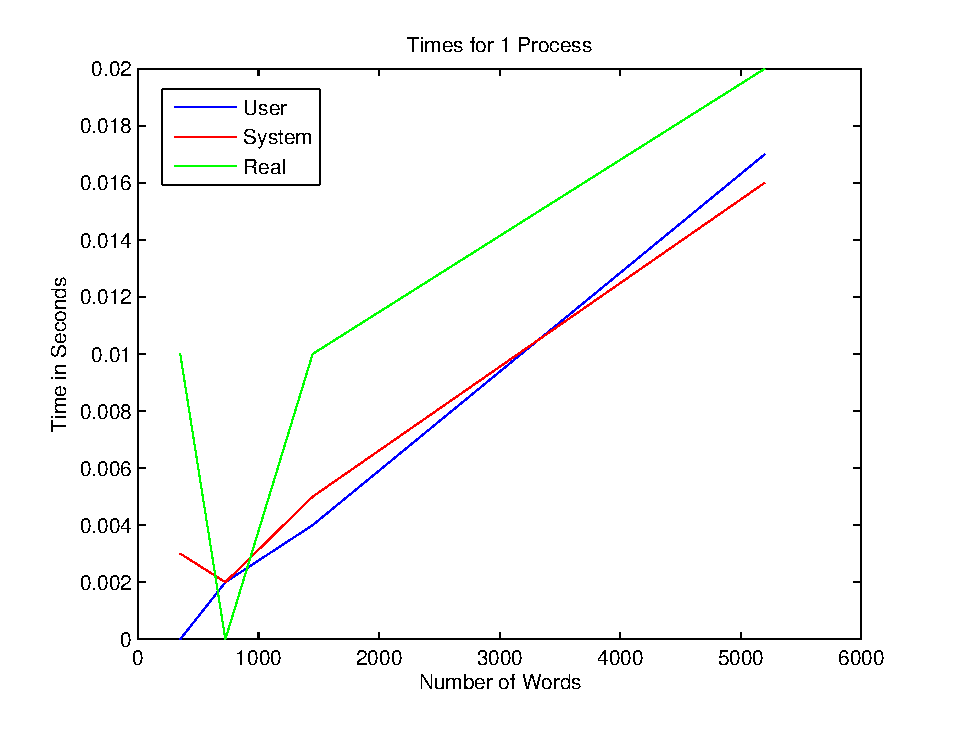
\includegraphics[width=0.75\textwidth]{process_1.eps}}
\centerline{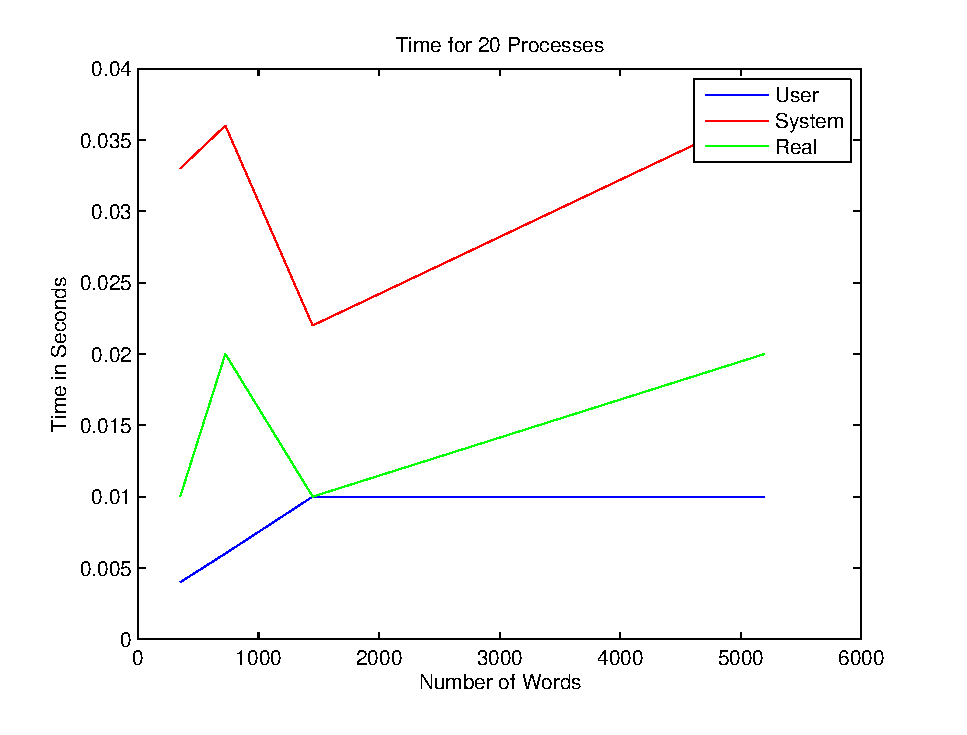
\includegraphics[width=0.75\textwidth]{process_20.eps}}
\centerline{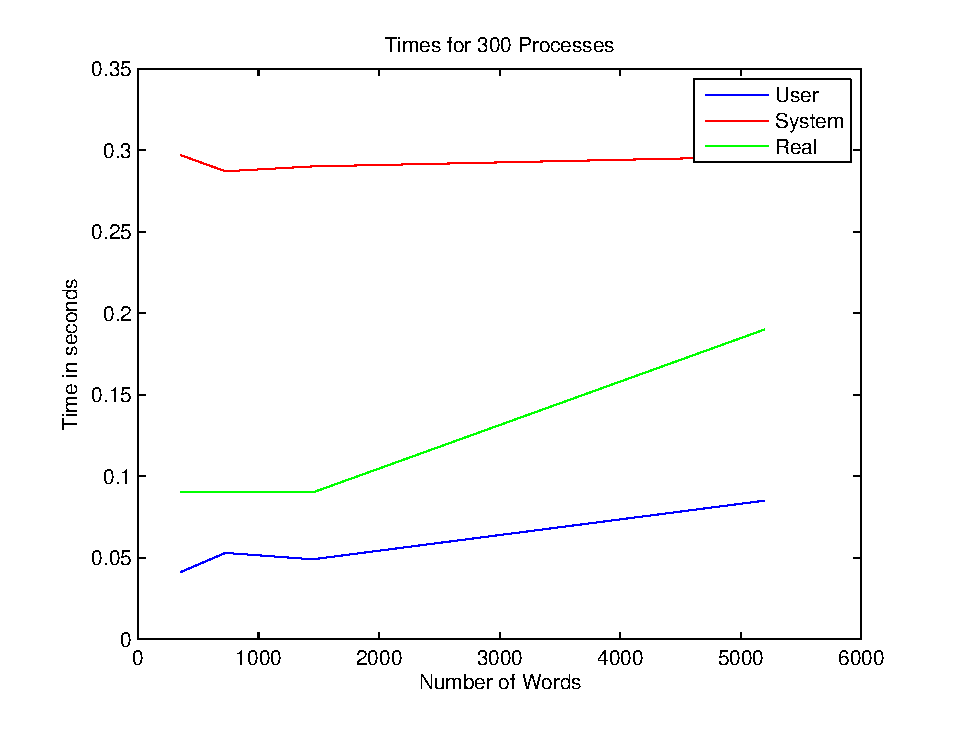
\includegraphics[width=0.75\textwidth]{process_300.eps}}
\centerline{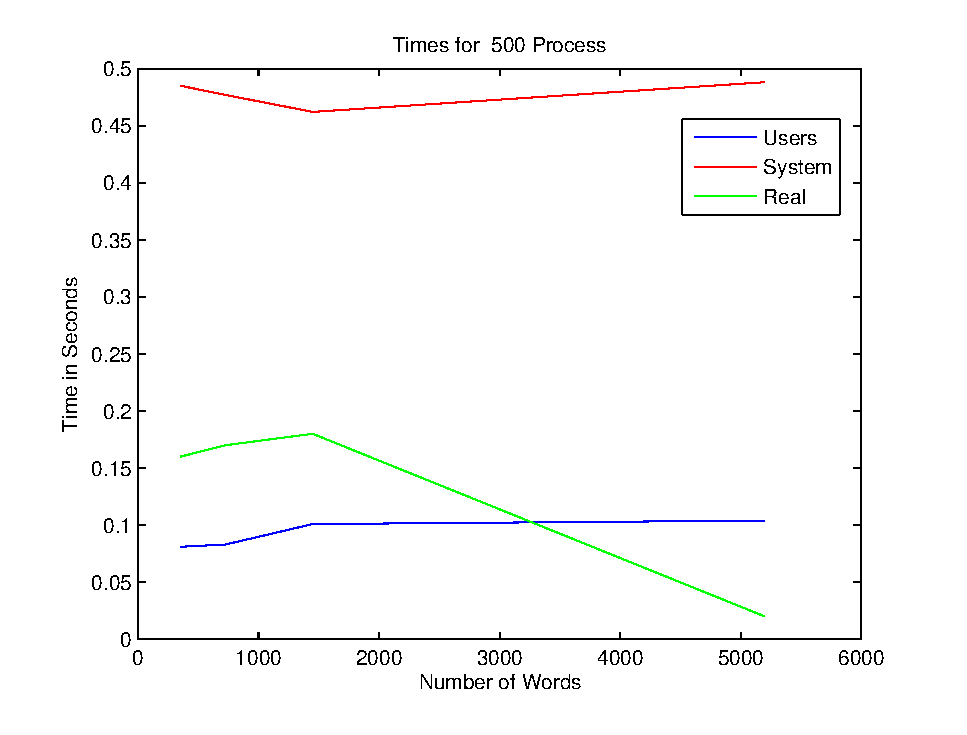
\includegraphics[width=0.75\textwidth]{process_500.eps}}


\section*{Challenges Overcame}
This program was very difficult for me conceptually. It was like my first time using pointers I was very confused
at first and dint quite understand them but hackishly made things work. That is kind of how I felt with pipes and
forking this assignment. It was quite hard to keep track of all of the file descriptors and at first. Another
challenge I faced was managing where each end of the pipes are and which need to be closed and opened that was
hard for me conceptually but after a few scribbles on a piece of paper I got my pipes and processes in running
order.. 
\section*{Questions}

\textbf{What do you think the main point of this assignment is?}\\
I think the main point of this assignment is to make us familiar with pipes and managing separate processes.
Pipes are used very often in the industry and are a very important concept to learn. I also believe that a point
of these assignments are to challenge us all and make us better programmers .
    
\textbf{How did you ensure your solution was correct?}\\
I verified my code by using a text file with no duplicate words. I would at first see how many words were in the
file with the command "cat input.txt | wc -w" this pipes the input file into a word counting utility and displays
how many words are in the file. Since i used no duplicate words I ran a my function with the same functionality
with the | wc -w command and it printed a list of all the words  and the same number exported from cat. I also
tested it with many other process numbers and different input file sizes. 
    
\textbf{What did you learn?}\\
I learned how to use Fork(), Pipes(), and Exec() this was the first time I have ever used any of these functions
and it was very interesting learning there functions and the workings. It was more difficult conceptually to
complete this assignment than it was to code.
    
\end{document}
